A continuación, se presenta la estructura dialógica en los textos visuales seleccionados, así como la identificación sistemática de las escenas que agrupan símbolos, signos denotativos, anacronismos e imágenes-síntoma. Se desarrolla la metodología indicada, se muestra la imagen seleccionada, se incluye un párrafo descriptivo y se lleva a cabo la categorización de los elementos visuales presentes en la imagen.

La categorización presentada en formato Mermaid responde a la necesidad de visualizar de manera clara y estructurada los conceptos clave de análisis de la imagen, que se basa en las ideas de \parencite{DidiHuberman2011}, Walter Benjamin y Rubén Dittus como se precisó en el capítulo anterior de metodología. El uso de Mermaid\footnote{Mermaid es una herramienta de código abierto que permite generar diagramas y gráficos a partir de texto en formato de marcado. Utiliza un lenguaje sencillo y legible para crear diagramas como diagramas de flujo, diagramas de secuencia, diagramas de clases, entre otros.} permite representar las relaciones entre las categorías de ``anacronismo'' e ``imagen síntoma'' de forma sencilla y accesible, facilitando la comprensión de cómo los diferentes elementos visibles en la imagen se agrupan y se interrelacionan. Este enfoque visual, además de ser una herramienta intuitiva para los análisis, refleja la naturaleza dinámica y compleja de los conceptos estudiados, promoviendo una reflexión más profunda sobre las conexiones temporales y simbólicas en la imagen.


\clearpage
\begin{figure}[h!]
    \centering
    \includegraphics[width=\textwidth]{AlaDeriva_diaz2016_fotograma-00-34-25.png}
    \caption{AlaDeriva diaz2016 fotograma 00:34:25}
    \label{fig:AlaDeriva_diaz2016_fotograma_00_34_25}
\end{figure}

Cocina de tamaño medio, con una ventana grande que ocupa casi toda una pared. La luz natural entra por la ventana, creando sombras y contrastes en los objetos. Una persona de espaldas cocinando en una estufa. Una mesa grande cubierta de objetos, incluyendo platos sucios, bolsas, botellas y papeles. En las paredes hay cuadros y utensilios de cocina colgados. Una mesa en primer plano llena de objetos. La encimera al fondo está llena de utensilios de cocina. \parencite[fotograma: 00:34:25]{AlaDeriva_diaz2016}

\small
\begin{verbatim}
    graph TD
    A[[Anacronismo]]
    B[[Imagen-Síntoma]]

    A --> A1[Desorden y caos en el espacio]
    A --> A2[Mezcla de objetos de diferentes épocas y usos]

    B --> B1[Acumulación de objetos]
    B --> B2[Posible situación de pobreza o precariedad]
    B --> B3[Salud mental]
\end{verbatim}
\normalsize

\clearpage
\begin{figure}[h!]
    \centering
    \includegraphics[width=\textwidth]{Citytv_junio2015_fotograma-00-00-16.png}
    \caption{Citytv junio2015 fotograma 00:00:16}
    \label{fig:Citytv_junio2015_fotograma_00_00_16}
\end{figure}

Fachada de un edificio con el letrero `ORTESIS Y PROTESIS'. Hay dos ventanas visibles: una parcialmente cubierta con plástico y una prenda blanca colgando, mientras que la otra tiene una tela clara con patrones color azul. Un cintillo de noticias rojo indica: "San Juan de Dios será entregado en tres fases" y "Distrito satisfecho tras la adquisición", mostrando además la hora 7:31 y los valores del dólar y el euro. Algunas personas aparecen parcialmente visibles en la esquina inferior izquierda. \parencite[fotograma: 00:00:16]{Citytv_junio2015}

\small
\begin{verbatim}
    graph TD
    A[[Anacronismo]]
    B[[Imagen-Síntoma]]
    
    A --> A1[Letrero "ORTESIS Y PROTESIS" en desuso]
    A --> A2[Arquitectura deteriorada]
    
    B --> B1[Exteriorización de hábitad humano]
    B --> B2[Contrqaste frase optimista y entorno desgastado]
    B --> B3[Afirmaciones oficiales subyacentes]
\end{verbatim}
\normalsize

\clearpage
\begin{figure}[h!]
    \centering
    \includegraphics[width=\textwidth]{AlaDeriva_diaz2016_fotograma-00-05-54.png}
    \caption{AlaDeriva diaz2016 fotograma 00:05:54}
    \label{fig:AlaDeriva_diaz2016_fotograma_00_05_54}
\end{figure}

Exterior del HSJD carrera décima vista hacia el sur. Se observa un vehículo blindado negro tipo antimotines con equipo de dispersión de agua en el techo. En primer plano, sobre el pavimento mojado, hay una persona vestida con bata blanca. Al fondo se distingue un grupo de policías con escudos antidisturbios formando una línea, mientras un chorro de agua es disparado hacia la derecha de la escena. \parencite[fotograma: 00:05:54]{AlaDeriva_diaz2016}

\small
\begin{verbatim}
graph TD
    A[[Anacronismo]]
    B[[Imagen-Síntoma]]
    
    A --> A1[Camión antimotines que evoca luchas sociales]
    A --> A2[Dotación antigua vs contexto inmutable]
    
    B --> B1[Calle concurrida refleja vida urbana]
    B --> B2[Mujer en aparente estado de calma vs presencia policial]
\end{verbatim}
\normalsize

\clearpage
\begin{figure}[h!]
    \centering
    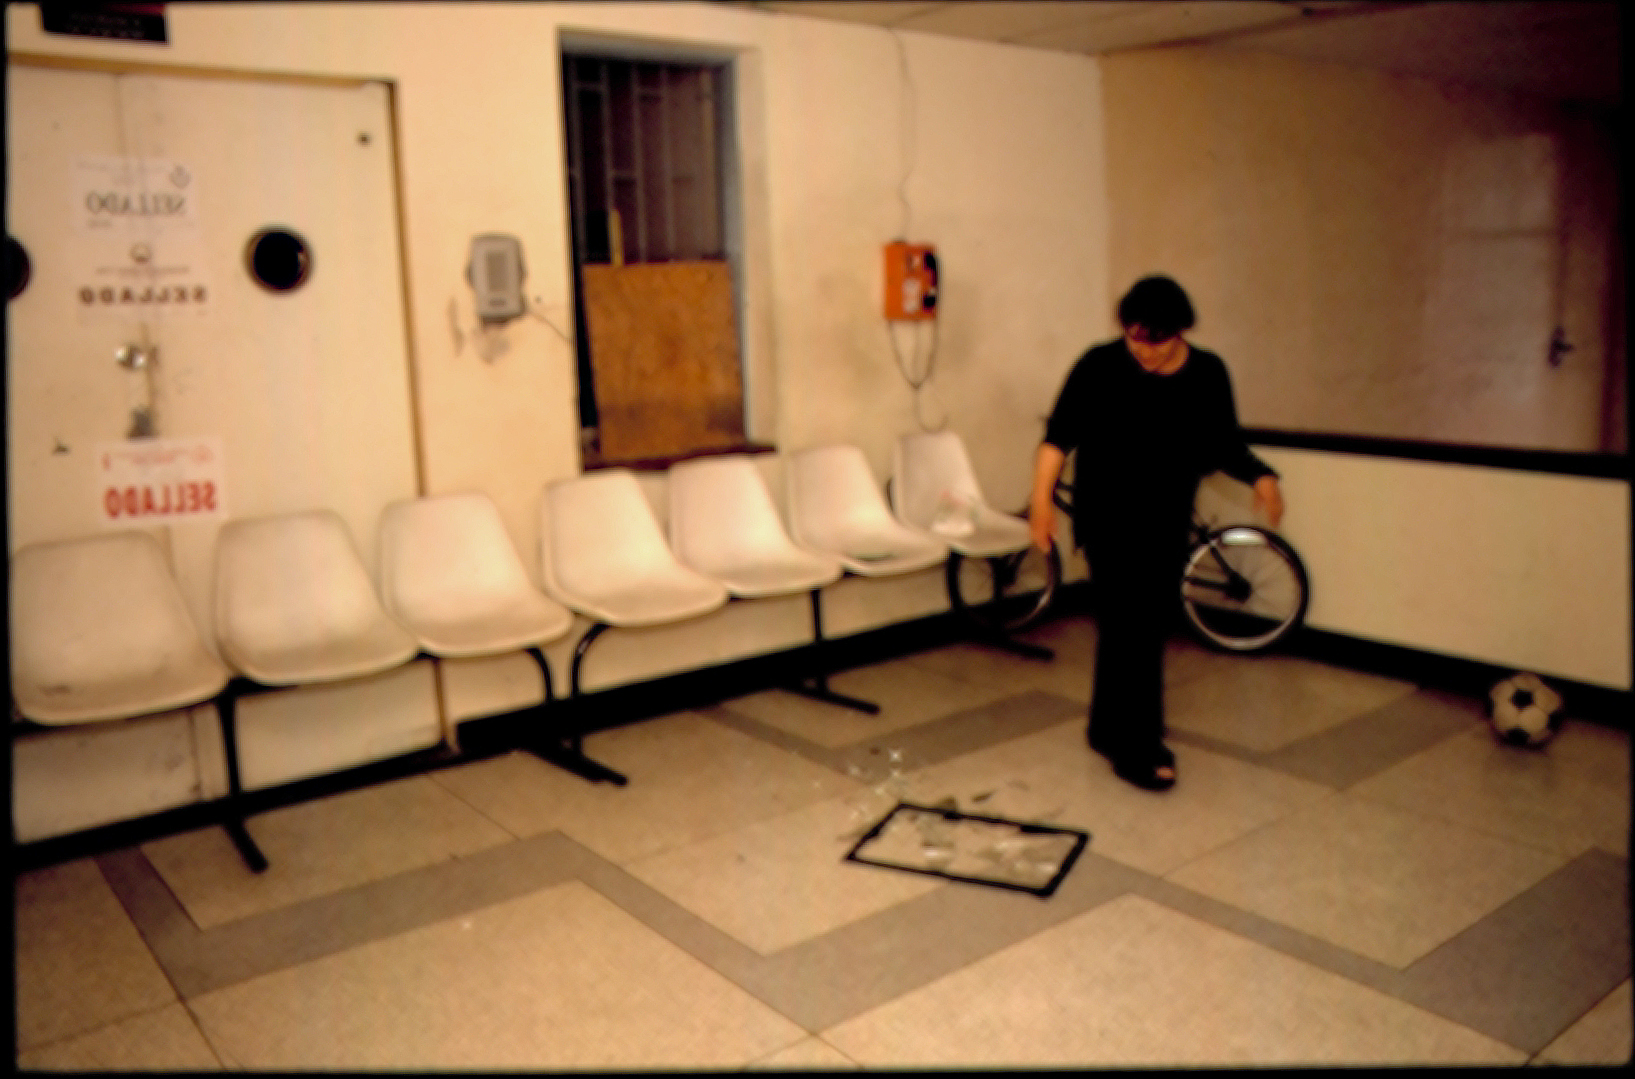
\includegraphics[width=\textwidth]{archivoMargarita_6octubre2004.jpg}
    \caption{Archivo Margarita 6 de octubre 2004}
    \label{fig:archivoMargarita_6octubre2004}
\end{figure}

Sala de espera con una fila de asientos blancos de plástico montados sobre una estructura metálica negra. La pared es de color crema claro con algunos elementos montados como un tablero y un teléfono naranja. El piso tiene un patrón geométrico en tonos beige y gris. En la escena hay una persona vestida de negro que mira hacia el suelo a lo que perece ser un marco y cristal rotos. Hay una bicicleta, un balón de fútbol y detrás de la hilera de sillas a la izquierda una puerta con letreros de `SELLADO'.

\small
\begin{verbatim}
graph TD
    A[[Anacronismo]]
    B[[Imagen-Síntoma]]
    
    A --> A1[Sala de espera vacía y austera]
    A --> A2[Uniformidad cromática en tonos desaturados]
    
    B --> B1[Soledad y aislamiento del individuo]
    B --> B2[Punctum visual elementos lúdicos]
    B --> B3[Deshumanización en espacios institucionales]
\end{verbatim}
\normalsize

\clearpage
\begin{figure}[h!]
    \centering
    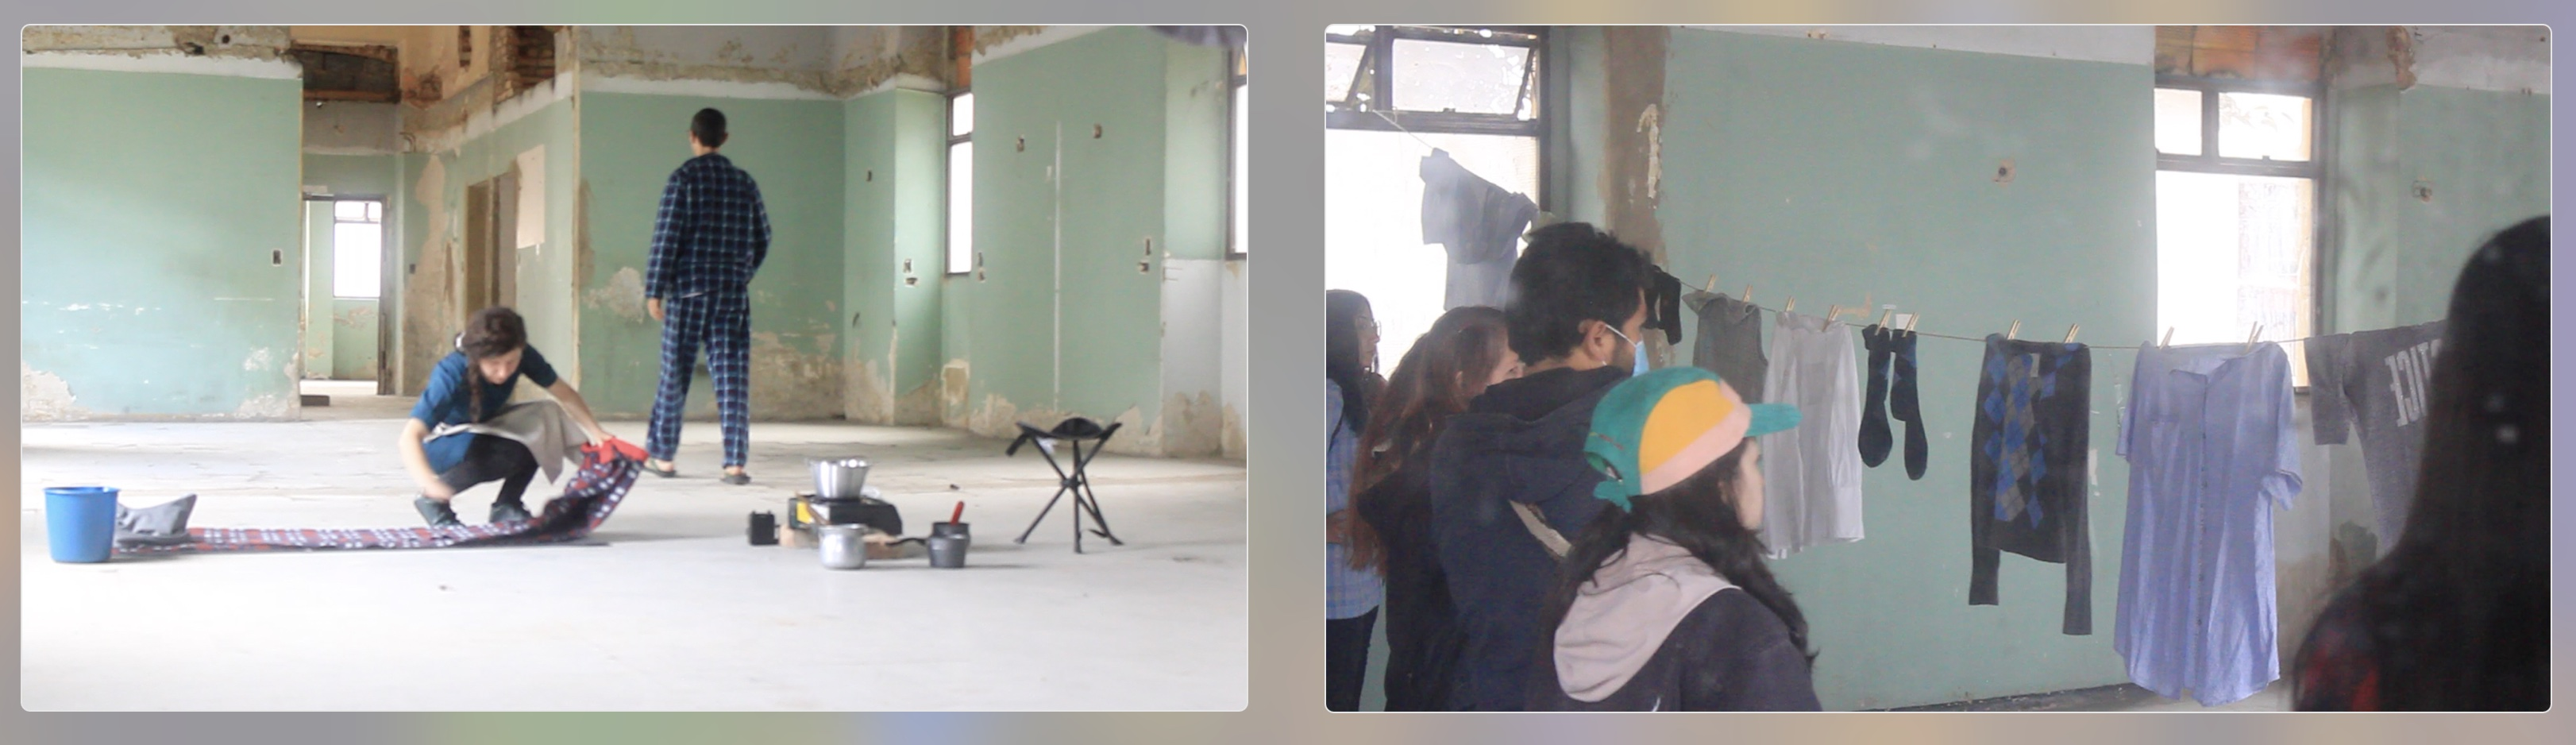
\includegraphics[width=\textwidth]{archivoJuanArroyo_10September2022_04_33.jpg}
    \caption{archivo Juan Arroyo 10 de Septiembre 2022}
    \label{fig:archivoJuanArroyo_10September2022_04_33}
\end{figure}

La imagen muestra edificio San Lucas en proceso de renovación o reparación. En la primera fotografía, se observan dos personas realizando tareas en el espacio - una sentada en el suelo trabajando con herramientas, y otra de pie observando. La segunda fotografía muestra a una persona sola de espaldas en el mismo espacio, se aprecia ropa colgada en una cuerda, dando la impresión de un espacio doméstico improvisado. Las paredes desgastadas, ventanas en crudo y suelo de concreto sugieren que el edificio está en una fase inacabada o de transición. Se yuxtaponen  escenas cotidianas de trabajo y vida dentro del entorno hospitalario.

\small
\begin{verbatim}
graph TD
    A[[Anacronismo]]
    B[[Imagen-síntoma]]

    A --> A1[Edificio San Lucas en renovación]
    A --> A2[Ropa colgada en una cuerda]
    A --> A3[Espacio doméstico improvisado]

    B --> B1[Personas habitando en contexto disruptivo]
    B --> B3[Paredes desgastadas y ventanas en crudo]
\end{verbatim}
\normalsize

\clearpage
\begin{figure}[h!]
    \centering
    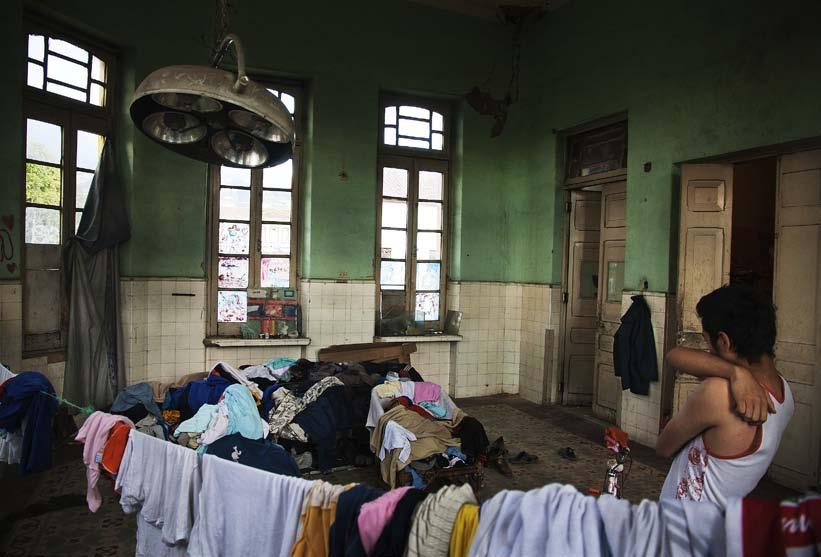
\includegraphics[width=\textwidth]{2011 Nicolas Van Hemelryck - San Juan sin Dios055.jpg}
    \caption{2011 Nicolas Van Hemelryck - San Juan sin Dios - 055}
    \label{fig:2011NicolasVanHemelryckSanJuansinDios-055}
\end{figure}

Sala de cirugía, interior deteriorado, ventanales que dejan entrar luz natural, contrastando con lámparas eléctricas colgantes. En este espacio se observan personas sentados en el piso sobre colchonetas y frazadas, rodeados de ropa y objetos personales. La escena revela síntomas de de usos disruptivos de ambiente para el cuidado quirúrjico y en hábitat doméstico. Foto del libro \parencite{Hemelryck2011}

\small
\begin{verbatim}
graph TD
    A[[Anacronismo]]
    B[[Imagen-Síntoma]]
    
    A --> A1[Modernidad caducada]
    A --> A2[Iluminación natural vs. ruinas de iluminación eléctrica]
    
    B --> B1[Gesto de relajación matutina]
    B --> B2[Acumulación sin orden de objetos personales]

\end{verbatim}
\normalsize